\documentclass[10pt]{beamer}
\usetheme{Boadilla}

\usepackage[T1]{fontenc}
\usepackage[utf8]{inputenc}
\usepackage{amsmath,amssymb,bm}
\usepackage{mathtools}
\usepackage{dsfont}
\usepackage{tikz}
\usetikzlibrary{arrows.meta,calc,positioning,decorations.pathreplacing}

\title[Distributional RL]{Distributional Reinforcement Learning | Part 2}
\author[Jonas Müller]{Jonas Müller}
\date{\today}

\newcommand{\R}{\mathbb{R}}
\newcommand{\E}{\mathbb{E}}
\newcommand{\Pcal}{\mathcal{P}}
\newcommand{\X}{\mathcal{X}}
\newcommand{\A}{\mathcal{A}}
\newcommand{\F}{\mathcal{F}}
\newcommand{\T}{\mathcal{T}}
\newcommand{\D}{\mathcal{D}}
\newcommand{\1}{\mathds{1}}
\newcommand{\norm}[1]{\lVert#1\rVert}

\begin{document}

\begin{frame}
  \titlepage
\end{frame}

\begin{frame}{Outline}
  \tableofcontents
\end{frame}

\section{Recap}

\begin{frame}{Recap: MDP and Return}
  We are working on a finite MDP: 
  \[
    (\X,\A,\xi_0,P_X,P_R),
    \qquad
    \pi:\X\to\Pcal(\A),
    \qquad
    \gamma\in[0,1).
  \]
  Trajectory process:
  \[
    X_0\sim\xi_0,\qquad
    A_t\sim\pi(\cdot\mid X_t),
  \]
  \[
    R_t\sim P_R(\cdot\mid X_t,A_t),
    \qquad
    X_{t+1}\sim P_X(\cdot\mid X_t,A_t),
    \qquad t\geq0.
  \]
  Discounted return:
  \[
    G^\pi(x)
    =
    \sum_{t=0}^{\infty}\gamma^t R_t
    \quad\text{given }X_0=x.
  \]
\end{frame}

\begin{frame}{Recap: Value function and Bellman Operator}
  The value function is given by the expected return: 
  \[
    V^\pi(x)=\E[G^\pi(x)] = \int_\R z\,d\eta_\pi(x)(z)
  \]
  Where $\eta_\pi(x) = \D(G^\pi(x))$ is the return distribution. \\

  As we know, there is a recursive relation for the value function known as Bellman's Equation: 
  \[
    V^\pi=\T^\pi V^\pi.
  \]
  Where we have the Bellman operator $\T^\pi:\R^\X\to\R^\X$:
  \[
    (\T^\pi V)(x)
    =
    \E_\pi\left[
      R+\gamma V(X')
      \mid X=x
    \right].
  \]

\end{frame}

\begin{frame}{Recap: Random-Variable Bellman Equation}
  With $(A,R,X')$ sampled from
  $\pi(\cdot\mid x)P_R(\cdot\mid x,A)P_X(\cdot\mid x,A)$,
  the random-variable Bellman equation is:
  \[
    G^\pi(x)
    \overset{D}{=}
    R+\gamma G^\pi(X')
    \mid X=x.
  \]
  Taking laws gives the return-distribution equation:
  \[
    \eta_\pi(x)
    =
    \D\left(R+\gamma G^\pi(X')\mid X=x\right).
  \]
  This is the distributional version of
  $(\T^\pi V)(x)=\E_\pi[R+\gamma V(X')\mid X=x]$.
\end{frame}

\begin{frame}{Recap: Distributional Bellman Operator}
  Define the bootstrap map
  \[
    b_{r,\gamma}(z)=r+\gamma z,
    \qquad r,z\in\R,
  \]
  and for $Z'\sim\eta(x')$,
  \[
    (b_{r,\gamma})_\#\eta(x')=\D(r+\gamma Z').
  \]
  Distributional Bellman operator $\T^\pi:\Pcal(\R)^\X\to\Pcal(\R)^\X$:
  \[
    (\T^\pi\eta)(x)
    =
    \E_\pi\left[
      (b_{R,\gamma})_\#\eta(X')
      \mid X=x
    \right].
  \]
  Distributional Bellman equation:
  \[
    \eta_\pi(x)
    =
    \E_\pi\left[
      (b_{R,\gamma})_\#\eta_\pi(X')
      \mid X=x
    \right],
    \qquad
    \eta_\pi=\T^\pi\eta_\pi.
  \]
\end{frame}

\begin{frame}{Recap: Representations of Return Distributions}
  Categorical representation:
  \[
    \eta(x)=\sum_{i=1}^m p_i^\theta(x)\delta_{\theta_i},
    \qquad
    p^\theta_i(x)\geq0,\quad \sum_{i=1}^m p_i^\theta(x)=1.
  \]
  Quantile representation:
  \[
    \eta(x)=\frac1m\sum_{i=1}^m\delta_{\theta_i(x)},
    \qquad
    \tau_i=\frac{2i-1}{2m},
    \qquad
    \theta_i(x)\approx F_{\eta(x)}^{-1}(\tau_i).
  \]
  \begin{block}{Focus of this Presentation} 
    If $\mathcal{X}$ is large, then storing even a scaler, let alone a distribution per state is expensive. 
    Hence, we look for suitable approximations.
  \end{block}
\end{frame}

\section{Scalar Linear Function Approximation}

\begin{frame}{Linear Value Function Approximation | Scalar Case}
  For weights $w\in\R^n$ approximate the value function as
  \[
    V_w(x)=\phi(x)^\top w,
    \qquad
    \nabla_w V_w(x)=\phi(x).
  \]
  For finite $\X$ and feature map $\phi$, stack feature rows into $\Phi\in\R^{|\X|\times n}$:
  \[
    V_w=\Phi w,
    \qquad
    \F_\phi=\{\Phi w:w\in\R^n\}.
  \]
  For state-action pairs, use e.g. $\phi:\X\times\A\to\R^n$ via
  $Q_w(x,a)=\phi(x,a)^\top w$.
  \begin{block}{Idea} 
    Instead of having a lookup table for the value of each state, we use a linear function to represent the function.
    \textcolor{red}{This function can be queried cheaply. }
  \end{block}

  \pause
  {\large\textcolor{red}{\textbf{Question}: How do we get a good $w$?}}
\end{frame}

\begin{frame}{Linear Approximation as Regression}
  Fitting a linear value function is just ordinary least squares:
  \[
    V_w=\Phi w,
    \qquad
    \min_{w\in\R^n}\norm{V^\pi-V_w}_{2}.
  \]

  which we could solve by the normal equation. 

  \begin{block}{However}
    In reinforcement learning, we might want to have a better approximation for some states than others.  
  \end{block}
\end{frame}


\begin{frame}{Weighted Norm for Linear Approximation}
  For some $\xi \in \Pcal(\X)$ we define the weighted $L_2$ norm and diagonal weight matrix
  \[
    \norm{V-V'}_{\xi,2}
    =\left(\sum_{x\in\X}\xi(x)(V(x)-V'(x))^2\right)^{1/2}.
    \qquad
    \Xi=\operatorname{diag}(\xi(x):x\in\X).
  \]

  The problem we now want to solve is: 
  $$
    \min_{w\in\R^n}\norm{V^\pi-V_w}_{\xi,2}.
  $$
  \pause
    \begin{block}{Proposition 9.3 $\mid$ Weighted Normal Equation}
    If $\xi$ has full support and the columns of $\Phi$ are linearly
    independent, the unique solution is
    \[
      w^*=(\Phi^\top\Xi\Phi)^{-1}\Phi^\top\Xi V^\pi.
    \]
  \end{block}
\end{frame}

\begin{frame}{Projection Back into the Feature Space}
  We have a linear approximation now, however we cant iterate the Bellman operator because we could have   
  $$\T^\pi V_w \notin \F_\phi$$. \\
  
  Define the weighted orthogonal projection
  \[
    (\Pi_{\phi,\xi}V)(x)=\phi(x)^\top w^*,
    \qquad
    w^*\in\arg\min_w\norm{V-V_w}_{\xi,2}.
  \]
  Approximate dynamic programming therefore iterates
  \[
    V_{k+1}=\Pi_{\phi,\xi}\T^\pi V_k.
  \]
  \begin{itemize}
    \item $\T^\pi$ performs the Bellman update.
    \item $\Pi_{\phi,\xi}$ removes components that the features cannot express.
  \end{itemize}
  Repeated projection can compound error (the diffusion effect).

\end{frame}

\begin{frame}{When Is the Projected Operator Stable?}
  Let $\xi_\pi$ be a fully supported steady-state distribution under $\pi$.
  \begin{block}{Projected Bellman contraction / Theorem 9.8}
    Since $P^\pi$ and $\Pi_{\phi,\xi_\pi}$ are nonexpansions in
    $\norm{\cdot}_{\xi_\pi,2}$,
    \[
      \norm{\Pi_{\phi,\xi_\pi}\T^\pi V-
      \Pi_{\phi,\xi_\pi}\T^\pi V'}_{\xi_\pi,2}
      \leq\gamma\norm{V-V'}_{\xi_\pi,2}.
    \]
  \end{block}
  Therefore there is a unique fixed point
  $\widehat V^\pi=\Pi_{\phi,\xi_\pi}\T^\pi\widehat V^\pi$, with
  \[
    \norm{\widehat V^\pi-V^\pi}_{\xi_\pi,2}
    \leq\frac{1}{\sqrt{1-\gamma^2}}
    \norm{\Pi_{\phi,\xi_\pi}V^\pi-V^\pi}_{\xi_\pi,2}.
  \]
\end{frame}

\begin{frame}{Scalar Linear Approximation: Proof Chain}
  The scalar argument works because everything lives in a Hilbert space:
  \[
    \R^\X,\qquad
    \langle V,V'\rangle_{\xi_\pi}
    =\sum_{x\in\X}\xi_\pi(x)V(x)V'(x).
  \]
  The feature class $\F_\phi=\{\Phi w:w\in\R^n\}$ is a linear subspace.
  \begin{enumerate}
    \item $\Pi_{\phi,\xi_\pi}$ is an orthogonal projection, hence nonexpansive.
    \item Stationarity of $\xi_\pi$ makes $P^\pi$ nonexpansive in
      $\norm{\cdot}_{\xi_\pi,2}$.
    \item The Bellman operator is affine with linear part $\gamma P^\pi$.
  \end{enumerate}
  Therefore
  \[
    \Pi_{\phi,\xi_\pi}\T^\pi
    \quad\text{is a }\gamma\text{-contraction.}
  \]
\end{frame}

\begin{frame}{Temporal-Difference Learning: Sampled Bellman Updates}
  Computing the Bellman iterates is expensive because it requires the expectation over the next state and reward.
  Instead, TD learning uses the sampled one-step Bellman target
  \[
    r_k+\gamma V_w(x'_k).
  \]
  The TD error is target minus current prediction:
  \[
    \delta_k=r_k+\gamma V_w(x'_k)-V_w(x_k).
  \]
  Equivalently, TD minimizes the squared TD error
  \[
    L_k(w)=\frac12\delta_k^2
    =
    \frac12
    \left(r_k+\gamma V_w(x'_k)-V_w(x_k)\right)^2.
  \]
  In the semi-gradient step, only $V_w(x_k)$ is differentiated:
  \[
    w\leftarrow w+\alpha_k\delta_k\nabla_w V_w(x_k).
  \]
  For linear features $V_w(x)=\phi(x)^\top w$:
  \[
    w\leftarrow w+\alpha_k\delta_k\phi(x_k).
  \]
\end{frame}

\begin{frame}{Section 9.4: Semi-Gradient TD}
  The book first writes the linear TD update as
  \[
    w \leftarrow w+\alpha_k
    \underbrace{\left(
      r_k+\gamma\phi(x'_k)^\top w-\phi(x_k)^\top w
    \right)}_{\text{TD error}}
    \phi(x_k).
  \]
  Then introduce a separate vector $\widetilde w$ in the target:
  \[
    w \leftarrow w+\alpha_k
    \left(
      r_k+\gamma\phi(x'_k)^\top\widetilde w-\phi(x_k)^\top w
    \right)\phi(x_k).
  \]
  With fixed $\widetilde w$, this is SGD on the sample loss and its solution
  satisfies
  \[
    \Phi w^*
    =
    \Pi_{\phi,\xi}\T^\pi V_{\widetilde w}.
  \]
  \begin{block}{Book's fixed-point statement}
    At the fixed point $\widehat V^\pi=\Phi\widehat w$ of the projected operator,
    \[
      \E_\pi\!\left[
      \left(
        R+\gamma\phi(X')^\top\widehat w-\phi(X)^\top\widehat w
      \right)\phi(X)
      \right]=0.
    \]
  \end{block}
\end{frame}

\begin{frame}{From Value function approximation to Distributional Approximation}
  Want to linearly approximate probability distributions. However in general 
  \[
   \eta_{w_1}(x)+\eta_{w_2}(x) \notin \Pcal(\R)
  \]
  and since the distribution lives in $\Pcal(\R)$, we can have non finite support. 
  \begin{block}{How to solve this?}
    Fix a finite dimensional family of distributions $\F_\theta\subset\Pcal(\R)$ and then linearly approximate the parameters of the distribution.
    ``Linear'' distributional approximation means that the \emph{parameters of
    a probability representation} depend linearly on features $\phi$.
  \end{block}
  There are therefore two approximation layers:
  \begin{enumerate}
    \item a finite probability representation (categorical or quantile),
    \item linear value function approximation.
  \end{enumerate}
\end{frame}

\begin{frame}{Finite Return-Distribution Families}
  For a probability measure $\eta\in\Pcal(\R)$, we have 
  \[
    F_\eta(t)=\eta((-\infty,t]),
    \qquad
    F_\eta^{-1}(\tau)=\inf\{z\in\R:F_\eta(z)\geq\tau\}.
  \]
  We consider the finite dimensional approximations:
  \[
    \text{categorical:}\qquad
    \eta(x)=\sum_{i=1}^m p_i(x)\delta_{\theta_i},
    \qquad
    p_i(x)\geq0,\quad \sum_{i=1}^m p_i(x)=1,
  \]
  \[
    \text{quantile:}\qquad
    \eta(x)=\frac1m\sum_{i=1}^m\delta_{\theta_i(x)},
    \qquad
    \tau_i=\frac{2i-1}{2m}, \qquad  \theta_i(x)\approx F_{\eta(x)}^{-1}(\tau_i).
  \]
  \begin{block}{What is state-dependent?}
    Categorical representations fix $\theta_i$ and learn the
    probabilities $p_i(x)$. Quantile fixes equal probabilities $1/m$ and learns
    locations $\theta_i(x)\approx F_{\eta(x)}^{-1}(\tau_i)$. \\

    \pause 
    \textcolor{red}{\textbf{Question}: We do not know $F^{-1}_{\eta(x)}$ in practice.}
  \end{block}
\end{frame}

\begin{frame}{Categorical vs. Quantile}
  \begin{columns}[T,onlytextwidth]
    \begin{column}{0.48\textwidth}
      \centering
      \textbf{Categorical}
      \[
        \eta(x)=\sum_{i=1}^m p_i(x)\delta_{\theta_i}
      \]
      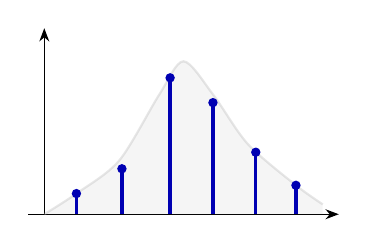
\begin{tikzpicture}[x=0.68cm,y=1.05cm,>=Stealth,
          every node/.style={font=\scriptsize}]
        \draw[->] (-2.9,0) -- (2.9,0);
        \draw[->] (-2.6,0) -- (-2.6,2.25);
        \fill[gray!35,opacity=0.22]
          plot[smooth] coordinates {(-2.6,0) (-2.0,0.25) (-1.2,0.65)
          (-0.45,1.45) (0.0,1.85) (0.55,1.45) (1.2,0.85)
          (2.1,0.35) (2.6,0.12)}
          -- (2.6,0) -- cycle;
        \draw[gray!55,opacity=0.35,thick]
          plot[smooth] coordinates {(-2.6,0) (-2.0,0.25) (-1.2,0.65)
          (-0.45,1.45) (0.0,1.85) (0.55,1.45) (1.2,0.85)
          (2.1,0.35) (2.6,0.12)};
        \foreach \x/\h in {-2.0/0.25,-1.15/0.55,-0.25/1.65,0.55/1.35,1.35/0.75,2.1/0.35} {
          \draw[very thick,blue!70!black] (\x,0) -- (\x,\h);
          \fill[blue!70!black] (\x,\h) circle (1.7pt);
        }
      \end{tikzpicture}
    \end{column}
    \begin{column}{0.48\textwidth}
      \centering
      \textbf{Quantile}
      \[
        \eta(x)=\frac1m\sum_{i=1}^m\delta_{\theta_i(x)}
      \]
      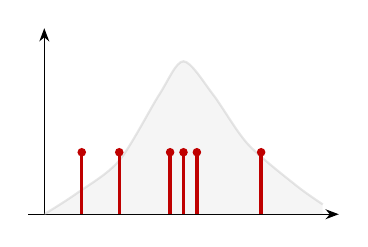
\begin{tikzpicture}[x=0.68cm,y=1.05cm,>=Stealth,
          every node/.style={font=\scriptsize}]
        \draw[->] (-2.9,0) -- (2.9,0);
        \draw[->] (-2.6,0) -- (-2.6,2.25);
        \fill[gray!35,opacity=0.22]
          plot[smooth] coordinates {(-2.6,0) (-2.0,0.25) (-1.2,0.65)
          (-0.45,1.45) (0.0,1.85) (0.55,1.45) (1.2,0.85)
          (2.1,0.35) (2.6,0.12)}
          -- (2.6,0) -- cycle;
        \draw[gray!55,opacity=0.35,thick]
          plot[smooth] coordinates {(-2.6,0) (-2.0,0.25) (-1.2,0.65)
          (-0.45,1.45) (0.0,1.85) (0.55,1.45) (1.2,0.85)
          (2.1,0.35) (2.6,0.12)};
        \foreach \x in {-1.9,-1.2,-0.25,0.0,0.25,1.45} {
          \draw[very thick,red!75!black] (\x,0) -- (\x,0.75);
          \fill[red!75!black] (\x,0.75) circle (1.55pt);
        }
      \end{tikzpicture}
    \end{column}
  \end{columns}
  \vspace{0.4em}
  \begin{block}{Key distinction}
    $\tau_i$ is a fixed probability level. $\theta_i(x)$ is the return value
    placed at that level.
  \end{block}
\end{frame}

\begin{frame}{Quantile Levels: Input $\tau$, Output $\theta$}
  \centering
  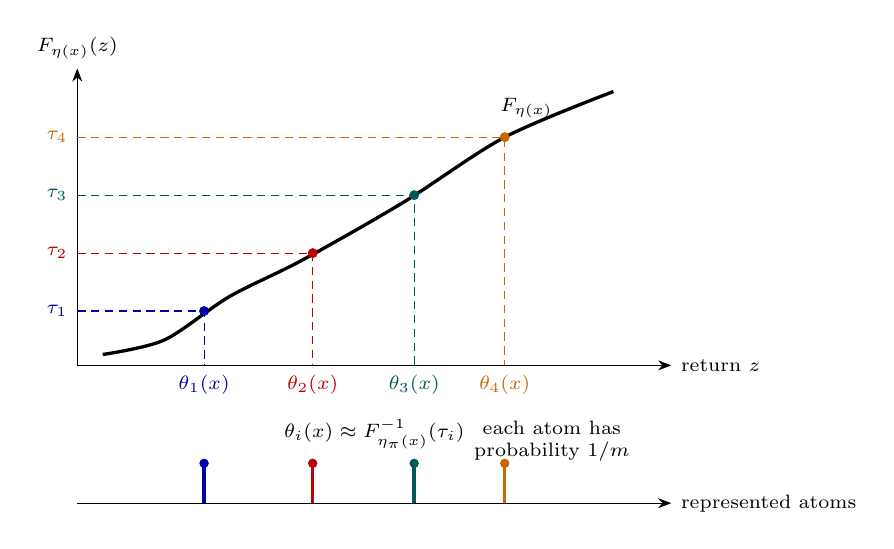
\begin{tikzpicture}[x=0.92cm,y=0.92cm,>=Stealth,
      every node/.style={font=\scriptsize}]
    \draw[->] (0,0) -- (8.2,0) node[right] {return $z$};
    \draw[->] (0,0) -- (0,4.1) node[above] {$F_{\eta(x)}(z)$};

    \draw[very thick,black]
      plot[smooth] coordinates {(0.35,0.15) (1.2,0.35) (2.1,0.95)
      (3.1,1.45) (4.5,2.25) (5.9,3.15) (7.4,3.78)};
    \node[black] at (6.2,3.55) {$F_{\eta(x)}$};

    \draw[densely dashed,blue!65!black] (0,0.75) -- (1.75,0.75) -- (1.75,0);
    \fill[blue!65!black] (1.75,0.75) circle (1.8pt);
    \node[left,blue!65!black] at (0,0.75) {$\tau_1$};
    \node[below,blue!65!black] at (1.75,0) {$\theta_1(x)$};

    \draw[densely dashed,red!75!black] (0,1.55) -- (3.25,1.55) -- (3.25,0);
    \fill[red!75!black] (3.25,1.55) circle (1.8pt);
    \node[left,red!75!black] at (0,1.55) {$\tau_2$};
    \node[below,red!75!black] at (3.25,0) {$\theta_2(x)$};

    \draw[densely dashed,teal!70!black] (0,2.35) -- (4.65,2.35) -- (4.65,0);
    \fill[teal!70!black] (4.65,2.35) circle (1.8pt);
    \node[left,teal!70!black] at (0,2.35) {$\tau_3$};
    \node[below,teal!70!black] at (4.65,0) {$\theta_3(x)$};

    \draw[densely dashed,orange!80!black] (0,3.15) -- (5.9,3.15) -- (5.9,0);
    \fill[orange!80!black] (5.9,3.15) circle (1.8pt);
    \node[left,orange!80!black] at (0,3.15) {$\tau_4$};
    \node[below,orange!80!black] at (5.9,0) {$\theta_4(x)$};

    \node[align=center] at (4.1,-0.95)
      {$\theta_i(x)\approx F_{\eta_\pi(x)}^{-1}(\tau_i)$};

    \begin{scope}[yshift=-1.75cm]
      \draw[->] (0,0) -- (8.2,0) node[right] {represented atoms};
      \draw[very thick,blue!65!black] (1.75,0) -- (1.75,0.55);
      \fill[blue!65!black] (1.75,0.55) circle (1.7pt);
      \draw[very thick,red!75!black] (3.25,0) -- (3.25,0.55);
      \fill[red!75!black] (3.25,0.55) circle (1.7pt);
      \draw[very thick,teal!70!black] (4.65,0) -- (4.65,0.55);
      \fill[teal!70!black] (4.65,0.55) circle (1.7pt);
      \draw[very thick,orange!80!black] (5.9,0) -- (5.9,0.55);
      \fill[orange!80!black] (5.9,0.55) circle (1.7pt);
      \node[align=center] at (6.55,0.85) {each atom has\\probability $1/m$};
    \end{scope}
  \end{tikzpicture}

  \vspace{0.6em}
  Changing $\tau_i$ asks for a different probability level; changing
  $\theta_i(x)$ moves the atom and therefore changes the represented
  distribution.
\end{frame}

\begin{frame}{Distributional TD: Learning}
  For fixed feature map $\phi(x)\in\mathbb R^d$.
  A linear method has, for every atom,  
  \[
    u_i(x)=\phi(x)^\top w_i,\qquad w_i\in\mathbb R^d.
  \]
  Observing a transition $(x,r,x')$ gives us a empirical target. We fit this via 
  \[
    w_i \leftarrow w_i+\alpha\,\varepsilon_i(x,r,x')\,\phi(x).
  \]
   where $\varepsilon_i$ is a error term. \textcolor{blue}{This term and the meaning of $u_i$ is what changes.}
\end{frame}

\begin{frame}{Linear Quantile TD: Representation and Loss}
  For the quantile representation, we choose 
  \[
    u_i(x) = \theta_i(x) = \phi(x)^\top w_i,
  \]
  The represented return distribution is
  \[
    \eta_w(x)=\frac1m\sum_{i=1}^m\delta_{\theta_i(x)}
    =
    \frac1m\sum_{i=1}^m\delta_{\phi(x)^\top w_i},
  \]
  Then we take the quantile loss as in the tabular case
  \[
    \rho_\tau(\Delta)=\left|\1_{\{\Delta<0\}}-\tau\right||\Delta|.
  \]
  For one target $z$, atom $i$ uses this loss on the residual
  \[
    L_{\tau_i}(w_i)=\rho_{\tau_i}\bigl(z-\phi(x)^\top w_i\bigr),
  \]
  whose subgradient w.r.t. $w_i$ is
  $-(\tau_i-\1_{\{z<\phi(x)^\top w_i\}})\phi(x)$.
\end{frame}

\begin{frame}{Linear QTD: Distributional Semi-Gradient}
  Similar to the tabular case, for transition $(x,a,r,x')$ we get $m$ target samples
  \[
    g_j=r+\gamma\phi(x')^\top w_j,
    \qquad j=1,\ldots,m.
  \]
  For atom $i$, average the quantile loss over these targets:
  \[
    L_i(w_i)=\frac1m\sum_{j=1}^m
    \rho_{\tau_i}\left(g_j-\phi(x)^\top w_i\right).
  \]
  The semi-gradient step is
  \[
    w_i
    \leftarrow
    w_i-\alpha\nabla_{w_i}L_i(w_i)
    =
    w_i+\alpha\frac1m\sum_{j=1}^m
    \underbrace{\left(\tau_i-
    \1_{\{g_j<\phi(x)^\top w_i\}}\right)}_{\text{quantile TD error}}
    \phi(x).
  \]
  %As in scalar TD, $g_j$ is treated as constant during differentiation.
  Unlike the scalar TD error, each averaged quantile error is in $ [-1,1]$.
\end{frame}

\begin{frame}{Linear Categorical TD: Prediction}
  We approximate the probabilites $p_i(x;w)$ by a linear combination of features:
  \[
    p_i(x;w)=
    \frac{\exp(\phi(x)^\top w_i)}
         {\sum_{j=1}^m\exp(\phi(x)^\top w_j)},
    \qquad
    \eta_w(x)=\sum_{i=1}^m p_i(x;w)\delta_{\theta_i}.
  \]
  transformed into probabilities by the softmax function. 
  Softmax is needed, direct linear coefficients need not be nonnegative or sum to one. 

  \pause 
  \begin{center}
      \textcolor{red}{This can be handled, later!}
        \end{center}

\end{frame}

\begin{frame}{Linear CTD: How to Stay on Fixed Support}
  \small
  For a sampled transition $(x,r,x')$, the Bellman update is an update
  of the prediction at the current state $x$:
  \[
    \underbrace{
    \eta_w(x)
    =
    \sum_{j=1}^m p_j(x;w)\delta_{\theta_j}
    }_{\text{prediction at }x}
    \xrightarrow{\quad \text{Observed }(r,x')\quad}
    \underbrace{
    (b_{r,\gamma})_\#\eta_w(x')
    =
    \sum_{j=1}^m p_j(x';w)\delta_{r+\gamma\theta_j}
    }_{\text{Empirical Bellman step for }x}.
  \]
  Since in general $r+\gamma\theta_j$ need not lie on the fixed support, use
  the categorical projection $\Pi_c$ to project the shifted atoms back to the fixed support
  $S=\{\theta_1,\ldots,\theta_m\}$.
  For each $j$,
  if $\theta_\ell\le r+\gamma\theta_j\le\theta_{\ell+1}$, split its mass as
  \[
    \bar p_\ell \mathrel{+}=
    p_j(x';w)\frac{\theta_{\ell+1}-(r+\gamma\theta_j)}
    {\theta_{\ell+1}-\theta_\ell},
    \qquad
    \bar p_{\ell+1} \mathrel{+}=
    p_j(x';w)\frac{(r+\gamma\theta_j)-\theta_\ell}
    {\theta_{\ell+1}-\theta_\ell}.
  \]
  This gives the projected target
   \[
    \bar\eta_{x,r,x'}
    =
    \Pi_c(b_{r,\gamma})_\#\eta_w(x')
    =\sum_{i=1}^m\bar p_i\delta_{\theta_i}.
  \]
\end{frame}

\begin{frame}{Linear CTD: Target, Loss, and Update}
  To learn softmax probabilities, we use the Cross-entropy loss:
  \[
    L(w)=-\sum_{i=1}^m\bar p_i\log p_i(x;w).
  \]
  Since
  \[
    \frac{\partial L}{\partial u_i}
    =
    p_i(x;w)-\bar p_i,
    \qquad
    \nabla_{w_i}u_i(x)=\phi(x),
  \]
  gradient descent gives the semi-gradient CTD update:
  \[
    w_i\leftarrow w_i+\alpha
    \underbrace{(\bar p_i-p_i(x;w))}_{\text{CTD error}}\phi(x).
  \]
\end{frame}

\begin{frame}{Chapter 9 Objects: Signed Categorical Family}
  We can make our lives to develop theory easier by allowing negative measures. 
  The signed categorical family on $S = \{\theta_1,\ldots,\theta_m\}$ is
  \[
    \F_{S,m}
    =
    \left\{
      \sum_{i=1}^m p_i\delta_{\theta_i}
      : p_i\in\R,\ \sum_{i=1}^m p_i=1
    \right\} \subseteq \mathcal M(\R).
  \]
  Using this we can define the signed categorical return functions
  \[
    \F_{S,m}^{\X}=\{\eta:\X\to\F_{S,m}\}.
  \]
  \pause
  \begin{center}
      \textcolor{red}{How to linearly approximate this?}
     \end{center}

\end{frame}

\begin{frame}{Chapter 9 Objects: Linear Signed Approximation}
  Linear approximation, subtracting the mean!
  \[
    p_i(x)
    =
    \frac1m
    +\phi(x)^\top w_i
    -\frac1m\sum_{j=1}^m\phi(x)^\top w_j .
  \]
  Then
  \[
    \sum_{i=1}^m p_i(x)=1,
    \qquad
    p_i(x)\in\R.
  \]
  The resulting family of distribution is denoted by $\F_{\phi,S,m}$.
  \pause
  \begin{center}
      \textcolor{red}{We want to perform bellman updates and ensure that the result is still in $\F_{\phi,S,m}$!}
  \end{center}
\end{frame}

\begin{frame}{Chapter 9 Objects: Why Two Projections?}
  \small
  Start with a $\eta\in\F_{\phi,S,m}$. After the Bellman update,
  \[
    \T^\pi\eta
  \]
  two things can go wrong.

  \medskip
  \textbf{1. Distribution representation.}
  For a state $x$, $(\T^\pi\eta)(x)$ need not be supported on
  $S=\{\theta_1,\ldots,\theta_m\}$. Hence we apply the categorical projection $\Pi_c$ from before. \\


  \textbf{2. Linear feature representation.}
  Even after $\Pi_c$, the map $x\mapsto(\Pi_c\T^\pi\eta)(x)$ need not lie in
  $\F_{\phi,S,m}$. Hence we need to define the feature projection by
  \[
    \Pi_{\phi,\xi,d}\widetilde\eta
    \in
    \arg\min_{\eta'\in\F_{\phi,S,m}}
    d(\widetilde\eta,\eta').
  \]
   In some suitable metric $d$. The final bellman update is then 
  \[
    \Pi_{\phi,\xi,d}\Pi_c\T^\pi\eta. \]
\end{frame}

\begin{frame}{Chapter 9 Objects: Cram\'er Geometry}
  We use the Cram\'er distance introduced prior, given by 
  \[
    \ell_2^2(\nu,\nu')
    =\int_\R\left(F_\nu(z)-F_{\nu'}(z)\right)^2\,dz
  \]
  whenever this quantity is finite. Define
  \[
    \mathcal M_{\ell_2,1}(\R)
    =
    \left\{
      \nu\in\mathcal M(\R):
      \nu(\R)=1,\ 
      \ell_2(\nu,\delta_0)<\infty
    \right\}.
  \]
  For return-distribution functions $\eta:\X\to\mathcal M_{\ell_2,1}(\R)$ we can again define a weighted distance
  \[
    \ell_{\xi,2}^2(\eta,\eta')
    =
    \sum_{x\in\X}\xi(x)
    \ell_2^2\!\left(\eta(x),\eta'(x)\right).
  \]
\end{frame}

\begin{frame}{Chapter 9 Lemmas: Bellman and Categorical Steps}
  Assume rewards have finite first moments and the Markov chain under $\pi$ has
  a unique stationary distribution $\xi_\pi$.
  \begin{block}{Lemma 9.14: Bellman Step}
    For any $\eta,\eta'\in\mathcal M_{\ell_2,1}(\R)^\X$,
    \[
      \ell_{\xi_\pi,2}(\T^\pi\eta,\T^\pi\eta')
      \leq
      \gamma^{1/2}\ell_{\xi_\pi,2}(\eta,\eta').
    \]
  \end{block}
  \begin{block}{Lemma 9.15: Categorical Projection}
    For any signed distributions $\nu,\nu'$,
    \[
      \ell_2(\Pi_c\nu,\Pi_c\nu')\leq \ell_2(\nu,\nu').
    \]
  \end{block}
\end{frame}

\begin{frame}{Chapter 9 Lemmas: Feature Projection}
  The final projection is the analogue of the scalar linear projection, but
  applied to signed categorical distributions with the Cram\'er metric.
  \begin{block}{Lemma 9.16: Linear Feature Projection}
    For any $\eta,\eta'\in\mathcal F_{S,m}^{\X}$,
    \[
      \ell_{\xi_\pi,2}
      \left(
        \Pi_{\phi,\xi_\pi,\ell_2}\eta,
        \Pi_{\phi,\xi_\pi,\ell_2}\eta'
      \right)
      \leq
      \ell_{\xi_\pi,2}(\eta,\eta').
    \]
  \end{block}
  Thus each piece is either a contraction or a nonexpansion:
  \[
    \T^\pi
    \quad\text{contracts,}\qquad
    \Pi_c,\ \Pi_{\psi,\xi_\pi,\ell_2}
    \quad\text{do not expand.}
  \]
\end{frame}

\begin{frame}{Chapter 9 Theorem: Doubly Projected Bellman}
  Composing the three preceding statements gives the actual convergence-style
  result for linear distributional approximation in the book.
  \begin{block}{Theorem 9.13}
    Under the assumptions above, for all
    $\eta,\eta'\in\mathcal M_{\ell_2,1}(\R)^\X$,
    \[
      \ell_{\xi_\pi,2}
      \left(
        \Pi_{\psi,\xi_\pi,\ell_2}\Pi_c\T^\pi\eta,
        \Pi_{\psi,\xi_\pi,\ell_2}\Pi_c\T^\pi\eta'
      \right)
      \leq
      \gamma^{1/2}\ell_{\xi_\pi,2}(\eta,\eta').
    \]
  \end{block}
  Hence the projected distributional Bellman operator has a unique fixed point
  in $\F_{\psi,S,m}$, by Banach's fixed-point theorem.
\end{frame}

\begin{frame}{Chapter 9: Exact Contraction Chain}
  For $\eta,\eta'\in\mathcal M_{\ell_2,1}(\R)^\X$,
  \[
  \begin{aligned}
    &\ell_{\xi_\pi,2}
    \left(
      \Pi_{\psi,\xi_\pi,\ell_2}\Pi_c\T^\pi\eta,
      \Pi_{\psi,\xi_\pi,\ell_2}\Pi_c\T^\pi\eta'
    \right) \\
    &\quad\leq
    \ell_{\xi_\pi,2}(\Pi_c\T^\pi\eta,\Pi_c\T^\pi\eta') \\
    &\quad\leq
    \ell_{\xi_\pi,2}(\T^\pi\eta,\T^\pi\eta') \\
    &\quad\leq
    \gamma^{1/2}\ell_{\xi_\pi,2}(\eta,\eta').
  \end{aligned}
  \]
  The three lines are exactly: feature projection nonexpansion,
  categorical projection nonexpansion, and distributional Bellman contraction.
\end{frame}

\section{Deep Distributional Reinforcement Learning}

\begin{frame}{From Fixed Features to Learned Features}
  A deep network replaces the hand-designed map $\phi(x)$ by a learned
  representation. Its penultimate layer can still be read as
  \[
    \phi_w(x)\in\R^n,
  \]
  followed by linear prediction heads.
  \begin{itemize}
    \item Earlier layers learn which state distinctions matter.
    \item Final layers map those features to values or distribution parameters.
    \item Backpropagation updates both simultaneously.
  \end{itemize}
  Linear approximation is therefore not discarded; it remains the final layer
  and the conceptual model for the deep semi-gradient update.
\end{frame}

\begin{frame}{From DQN to Distributional DQN}
  \small
  Standard DQN predicts one scalar per action:
  \[
    x\longmapsto \bigl(Q_w(x,a)\bigr)_{a\in\A},
    \qquad
    Q_w(x,a)\approx\E[Z(x,a)].
  \]
  Distributional DQN predicts a return distribution per action:
  \[
    x\longmapsto \bigl(\eta_w(x,a)\bigr)_{a\in\A},
    \qquad
    \eta_w(x,a)\approx \D(Z(x,a)).
  \]
  For a transition $(x,a,r,x')$, the target is now a shifted future-return
  distribution:
  \[
    (b_{r,\gamma})_\#\eta_{\widetilde w}(x',a^*),
    \qquad
    a^*\in\arg\max_{a'\in\A}Q_{\widetilde w}(x',a').
  \]
  The output has $m$ distribution parameters per action:
  \[
    x\longmapsto\R^{|\A|\times m}.
  \]
  \begin{itemize}
    \item \textbf{C51:} using the categorical representation
    \item \textbf{QR-DQN:} using the quantile representation
    \item \textbf{IQN:} quantile level $\tau$ becomes an additional input.
  \end{itemize}
\end{frame}

\begin{frame}{C51: Prediction and Behavior}
  Using state action categorical representation with fixed $\theta_1<\cdots<\theta_m$, the network outputs 
  $\phi_i(x,a;w)$ and
  \[
    p_i(x,a;w)=\frac{e^{\phi_i(x,a;w)}}
    {\sum_{j=1}^m e^{\phi_j(x,a;w)}},
    \qquad
    \eta_w(x,a)=\sum_{i=1}^mp_i(x,a;w)\delta_{\theta_i}.
  \]
  The induced action value is
  \[
    Q_w(x,a)=\sum_{i=1}^mp_i(x,a;w)\theta_i.
  \]
  Original C51 uses $m=51$ evenly spaced atoms.
\end{frame}

\begin{frame}{C51 Learning Algorithm}
  Select the target-network greedy action
  \[
    a_{\widetilde w}(x')\in\arg\max_{a'}Q_{\widetilde w}(x',a').
  \]
  Construct and project the target
  \[
    \bar\eta(x,a)=
    \Pi_c(b_{r,\gamma})_\#\eta_{\widetilde w}
    (x',a_{\widetilde w}(x'))
    =\sum_{j=1}^m\bar p_j\delta_{\theta_j}.
  \]
  Then minimize the cross entropy loss $L(w)=-\sum_{j=1}^m\bar p_j\log p_j(x,a;w)$ and update
  \[
    w\leftarrow w+\alpha
    \sum_{i = 1}^{m}  (\bar p_i-p_i(x;w)) \nabla_w \theta_i(x,y ; w).
  \]
  This is pretty much the same as the linear CTD update, aside from the need to update vector valued. 
\end{frame}

\begin{frame}{QR-DQN: Quantile Prediction}
  QR-DQN interprets the $m$ outputs as locations of an equally weighted
  quantile distribution:
  \[
    \eta_w(x,a)=\frac1m\sum_{i=1}^m\delta_{\theta_i(x,a;w)},
    \qquad
    Q_w(x,a)=\frac1m\sum_{i=1}^m\theta_i(x,a;w).
  \]
  With $a_{\widetilde w}(x')$ greedy by this mean, the pairwise residuals are
  \[
    \Delta_{ij}=r+\gamma\theta_j(x',a_{\widetilde w}(x');\widetilde w)
    -\theta_i(x,a;w).
  \]
  Every predicted quantile is compared with every target quantile.
\end{frame}

\begin{frame}{QR-DQN: Quantile Huber Loss}
  For $\tau_i=(2i-1)/(2m)$, QR-DQN minimizes
  \[
    L(w)=\frac1m\sum_{i,j=1}^m\rho^H_{\tau_i}(\Delta_{ij}),
    \qquad
    \rho^H_\tau(u)=|\1_{\{u<0\}}-\tau|H_1(u),
  \]
  where
  \[
    H_1(u)=
    \begin{cases}
      \frac12u^2,&|u|\leq1,\\
      |u|-\frac12,&|u|>1.
    \end{cases}
  \]

  \begin{block}{Difference to linear case}
    \begin{itemize}
      \item We use the Huber loss to reduce sensitivity to outliers and have a differentiable loss.
      \item The loss is over all weights simultaneously, not entrywise. 
    \end{itemize}
    
  \end{block}
\end{frame}


\begin{frame}{Takeaways}
  \begin{enumerate}
    \item Linear approximation introduces state aliasing and a weighted projection
      problem; the sampling distribution is central to stability.
    \item Semi-gradient TD tracks a projected Bellman process, and target weights
      make that relationship explicit.
    \item Linear QTD and CTD make distribution \emph{parameters} linear in features.
    \item Deep methods learn the features and retain the same prediction--target--
      semi-gradient structure.
    \item C51, QR-DQN, and IQN differ mainly in how they parameterize and train the
      output distribution; that choice also shapes the learned representation.
  \end{enumerate}
\end{frame}

\begin{frame}{References}
  \footnotesize
  \begin{itemize}
    \item Bellemare, Dabney, Rowland (2023): \emph{Distributional Reinforcement Learning}, Chapters 9--10.
    \item Bellemare, Dabney, Munos (2017): A Distributional Perspective on Reinforcement Learning.
    \item Dabney et al. (2018): Distributional Reinforcement Learning with Quantile Regression.
    \item Dabney et al. (2018): Implicit Quantile Networks for Distributional Reinforcement Learning.
  \end{itemize}
\end{frame}



\begin{frame}{Chapter 10: Why This Is Not a DQN Theorem}
  C51, QR-DQN, and IQN combine several ingredients:
  \[
    \text{nonlinear network}
    + \text{bootstrapping}
    + \text{greedy control}
    + \text{replay/target networks}.
  \]
  The theory is therefore much weaker than for policy evaluation.
  \begin{block}{What Theorem 9.13 needs}
    A fixed policy, linear projection in a fixed metric, and a fixed operator
    \[
      \Pi_{\psi,\xi_\pi,\ell_2}\Pi_c\T^\pi .
    \]
  \end{block}
  \begin{block}{What Chapter 10 uses}
    Nonlinear parameters and a moving control target, e.g.
    \[
      r+\gamma Z_{\widetilde w}
      \left(x',\arg\max_{a'}\E[Z_{\widetilde w}(x',a')]\right).
    \]
  \end{block}
  So Chapter 10 inherits the projection intuition, but not a comparable general
  convergence theorem for deep distributional DQN.
\end{frame}

\begin{frame}{IQN: Make the Quantile Level an Input}
  C51 and QR-DQN output a fixed finite parameter vector. IQN instead models
  the quantile function itself:
  \[
    (x,a,\tau)\longmapsto
    \theta_w(x,a,\tau)\approx F^{-1}_{\eta(x,a)}(\tau).
  \]
  The level is encoded by
  \[
    \varphi(\tau)=(\cos(\pi\tau i))_{i=0}^{M-1},
  \]
  transformed by a fully connected layer, and combined multiplicatively with
  the state features. The final action heads satisfy
  \[
    \theta_w(x,a,\tau)=\phi_w(x,\tau)^\top w_a.
  \]
\end{frame}

\begin{frame}{IQN: Behavior and Learning}
  Approximate the mean with independent $\tau_i\sim\mathcal U(0,1)$:
  \[
    Q_w(x,a)\approx\frac1m\sum_{i=1}^m\theta_w(x,a,\tau_i).
  \]
  For independent online levels $\tau_i$ and target levels $\tau'_j$, minimize
  pairwise losses of
  \[
    r+\gamma\theta_{\widetilde w}
      (x',a_{\widetilde w}(x'),\tau'_j)
    -\theta_w(x,a,\tau_i).
  \]
  Sampling many level pairs reduces gradient variance. IQN approximates the
  whole quantile function without committing to fixed output locations.
\end{frame}

\begin{frame}{IQN Makes Risk Sensitivity Simple}
  Risk-neutral behavior samples $\tau\sim\mathcal U(0,1)$. Lower-tail CVaR at
  level $\bar\tau$ is
  \[
    \operatorname{CVaR}_{\bar\tau}(G_w(x,a))
    =\frac1{\bar\tau}\int_0^{\bar\tau}\theta_w(x,a,\tau)\,d\tau.
  \]
  Approximate it by changing only the sampling distribution:
  \[
    \operatorname{CVaR}_{\bar\tau}(G_w(x,a))
    \approx\frac1m\sum_{i=1}^m\theta_w(x,a,\tau_i),
    \quad \tau_i\sim\mathcal U(0,\bar\tau).
  \]
  Thus an implicit representation separates learning the return distribution
  from choosing how that distribution should guide behavior.
\end{frame}

\begin{frame}{How Distributional Predictions Shape Features}
  Split the network into learned features and final prediction heads.
  \begin{itemize}
    \item DQN trains the representation to predict one conditional mean per action.
    \item C51 trains it through $m$ probability errors per action.
    \item QR-DQN/IQN train it through many pairwise quantile residuals.
  \end{itemize}
  The type and number of predictions therefore change the learned state
  representation. This richer auxiliary prediction problem is a leading
  explanation for improved control performance even when actions are ultimately
  selected by the mean.
\end{frame}


\end{document}
